\documentclass{beamer}
\usepackage[english,russian]{babel}
\usepackage[utf8]{inputenc}
\usepackage{amsmath}
\usepackage{hyperref}
\usetheme{Warsaw}
\usepackage{listings}
\usepackage{xcolor}
\usepackage{tikz}
\usetikzlibrary{graphs}
\usepackage{algorithm}
\usepackage{algpseudocode}

\lstset{
    frame=tb,
    tabsize=4,
    showstringspaces=false,
    numbers=left,
    commentstyle=\color{green},
    keywordstyle=\color{blue},
    stringstyle=\color{red},
    emph={baz},
    emphstyle=\textbf
}

\begin{document}

\title{SAT/SMT solvers\newline  2. Conflict-Driven Clause Learning algorithm}
\author{Roman Kholin}
\institute{Lomonosov Moscow State University}
\date{Moscow, 2023}

\begin{frame}
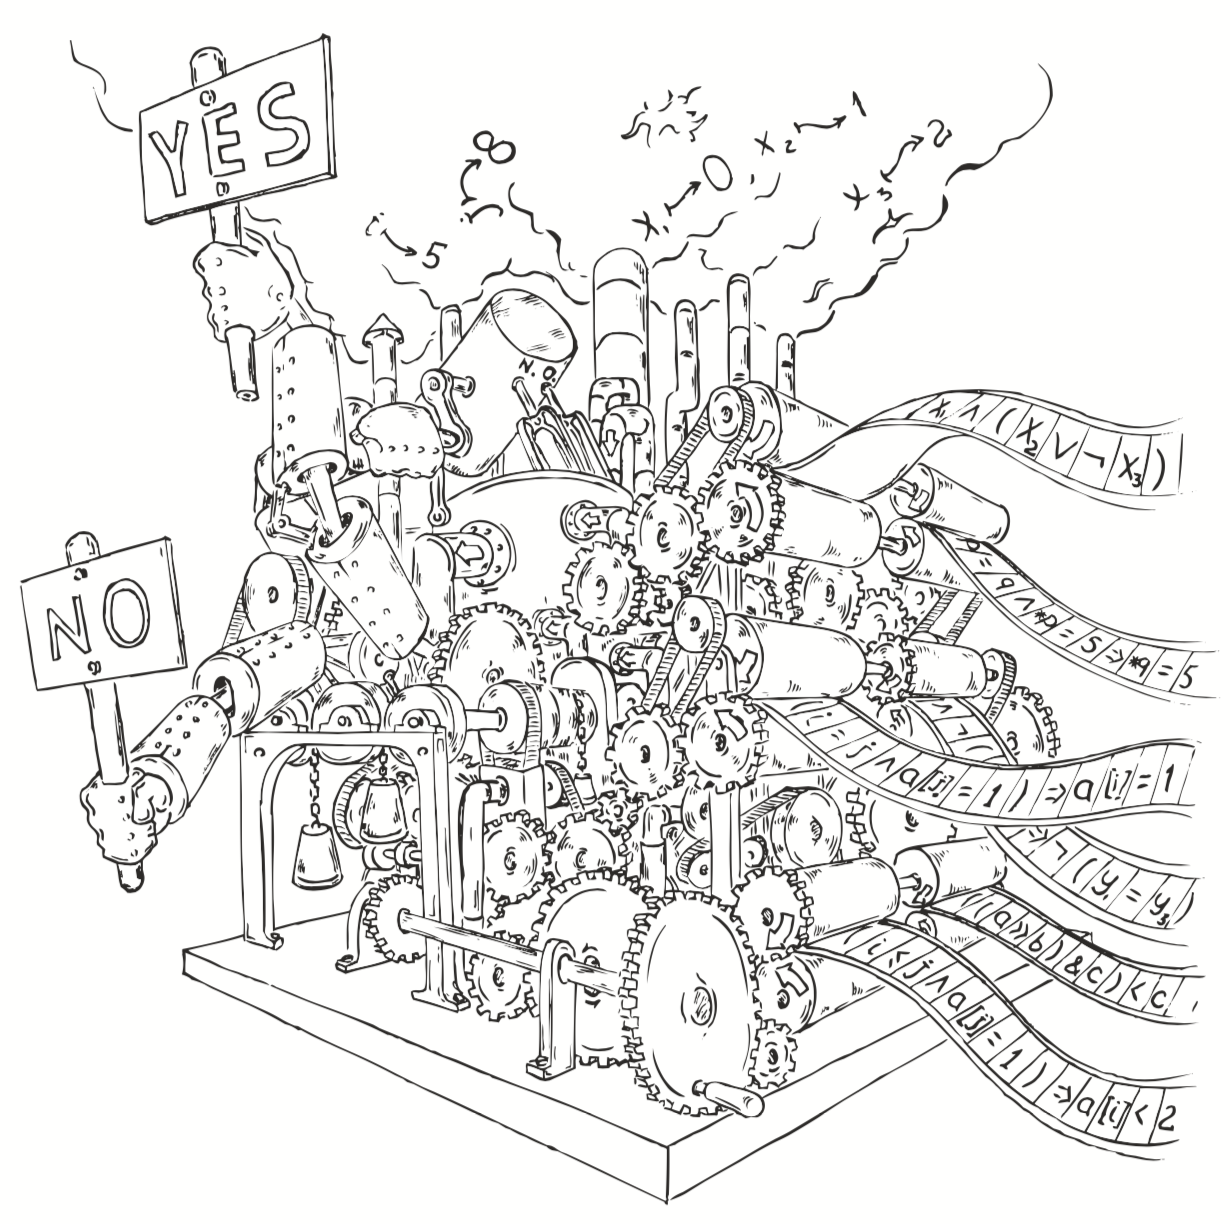
\includegraphics[scale=0.5]{../decision-procedure.png}
\end{frame}

\frame{\titlepage}

\begin{frame}{Obvious algorithm}
\begin{itemize}
\item Brute force
\item $O(2^n)$
\end{itemize}
\end{frame}

\begin{frame}{Definitions}
\begin{block}{State of a clause under an assignment}
A clause is satisfied if one or more of its literals are satisfied, conflicting if all of its literals are assigned but not satisfied, unit if it is not satisfied and all but one of its literals are assigned, and unresolved otherwise.
\end{block}
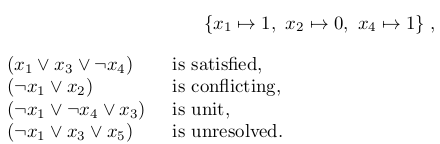
\includegraphics[scale=0.5]{assign.png}
\begin{block}{}
The clause $C := (\lnot x_1 \vee \lnot x_4 \vee x_3)$ and the partial assignment $\{x_1 \rightarrow 1, x_4 \rightarrow 1\}$ imply the assignment $x_3$ and $Antecedent(x_3) = C$
\end{block}
\end{frame}

\begin{frame}{Definitions}
\begin{block}{Implication graph}
An implication graph is a labeled directed acyclic graph G(V, E), where:
\begin{itemize}
\item V represents the literals of the current partial assignment (we refer to a node and the literal that it represents interchangeably). Each node is labeled with the literal that it represents and the decision level at which it entered the partial assignment
\item $E$ with $E = \{(v_i , v_j ) | v_i, v_j \in V, \lnot v_i \lnot Antecedent(v_j)\}$ denotes the set of directed edges where each edge $(v_i, v_j)$ is labeled with Antecedent($v_j$)
\item G can also contain a single conflict node labeled with k and incoming edges $\{(v, k) | \lnot v \in c\}$ labeled with c for some conflicting clause c
\end{itemize}
\end{block}
\end{frame}

\begin{frame}{Example}
$c_1 = (\lnot x_1 \vee x_2 )$\newline
$c_2 = (\lnot x_1 \vee x_3 \vee x_5 )$\newline
$c_3 = (\lnot x_2 \vee x_4 )$\newline
$c_4 = (\lnot x_3 \vee \lnot x_4 )$\newline
$c_5 = (x_1 \vee x_5 \vee \lnot x_2 )$\newline
$c_6 = (x_2 \vee x_3 )$\newline
$c_7 = (x_2 \vee \lnot x_3 )$\newline
$c_8 = (x_6 \vee \lnot x_5 )$\newline
Let $x_1@6$ and $\lnot x_5@3$
\end{frame}

\begin{frame}{Conflict-driven clause learning}
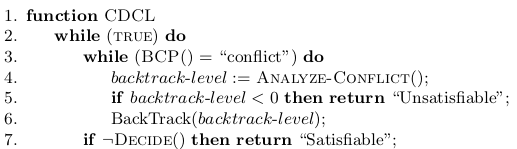
\includegraphics[scale=0.4]{CDCL.png}
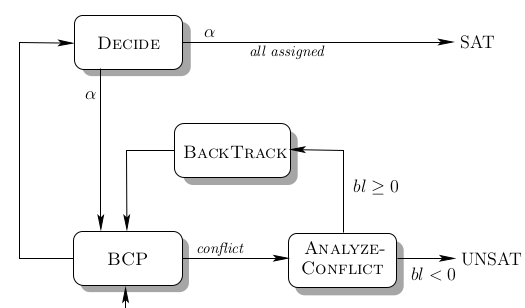
\includegraphics[scale=0.4]{CDCL_scheme.png}
\begin{block}{}
It is never the case that the solver enters decision level dl again with the same partial assignment
\end{block}
\end{frame}

\begin{frame}{}
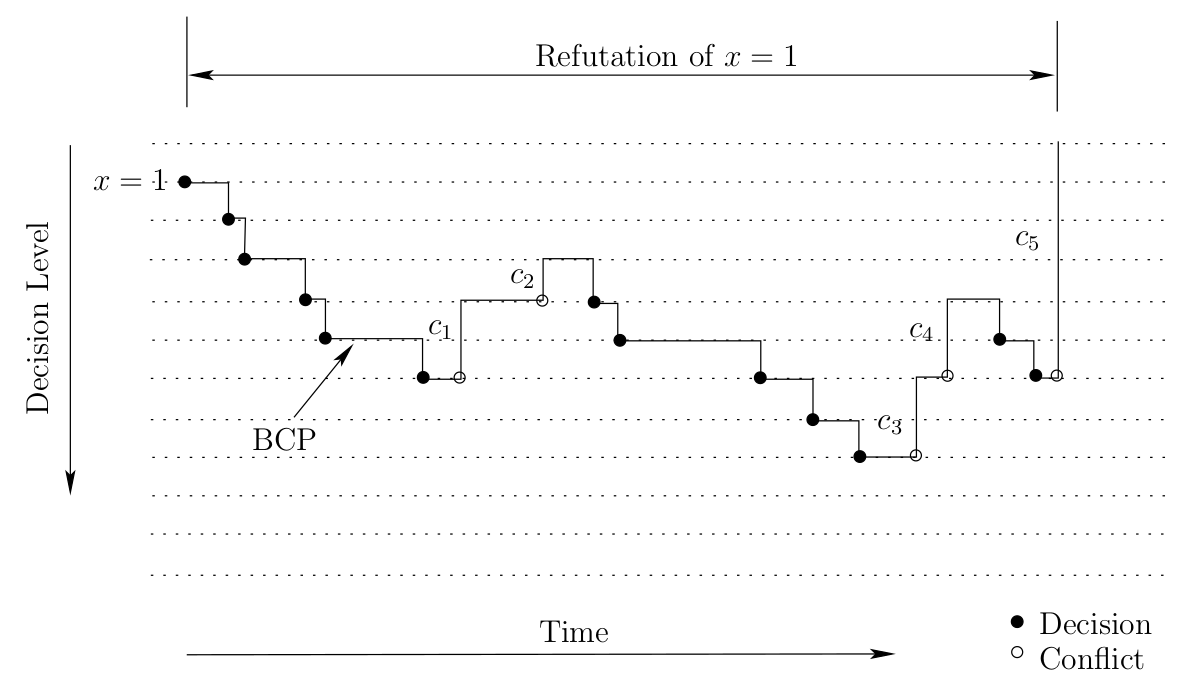
\includegraphics[scale=0.25]{Graph.png}
\end{frame}

\begin{frame}{UIP}
\begin{block}{Unique Implication Point (UIP)}
Given a partial conflict graph corresponding to the decision level of the conflict, a unique implication point (UIP) is any node other than the conflict node that is on all paths from the decision node to the conflict node
\end{block}
\begin{block}{First UIP}
A first UIP is a UIP that is closest to the conflict node
\end{block}
\end{frame}

\begin{frame}{UIP}
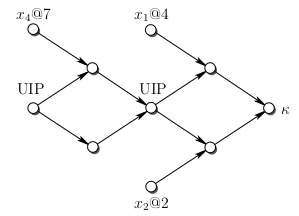
\includegraphics[scale=0.4]{UIP.png}
\begin{block}{Binary resolution and related terms}
\end{block}
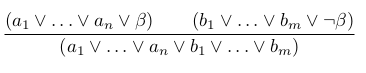
\includegraphics[scale=0.5]{Binary_resolution.png}
where $a_1, \dots, a_n, b_1, \dots, b_m$ are literals and $\beta$ is a variable. The variable $\beta$ is called the resolution variable. The clauses ($a_1 \vee \dots \vee a_n \vee \beta)$ and $(b_1 \vee \dots \vee b_m \vee (\lnot\beta))$ are the resolving clauses, and $(a_1 \vee \dots \vee a_n \vee b_1 \dots \vee b_m)$ is the resolvent clause
\end{frame}

\begin{frame}{Analyze conflict}
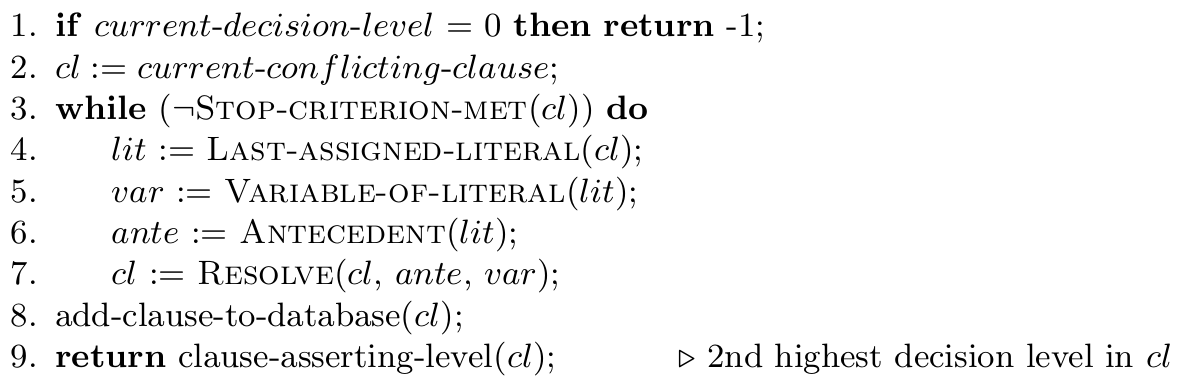
\includegraphics[scale=0.25]{Analyze-Conflict.png}\newline
Stop-criterion-met(cl) is to return true if and only if cl contains the negation of the first UIP as its single literal at the current decision level.\newline
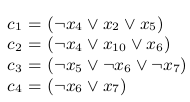
\includegraphics[scale=0.5]{UIP1.png}
\end{frame}

\begin{frame}{Decision Heuristics}
\begin{itemize}
\item Jeroslow–Wang: compute for each literal $l$\newline
$J(l) = \Sigma_{w \in B, l \in w}2^{-|w|}$
\item Dynamic Largest Individual Sum (DLIS): at each decision level, choose the unassigned literal that satisfies the largest number of currently unsatisfied clauses
\item Variable State Independent Decaying Sum (VSIDS): A new conflict clause, adds 1 to the score of each literal that appears in it. Periodically divide all scores by 2.
\end{itemize}
\end{frame}

\begin{frame}
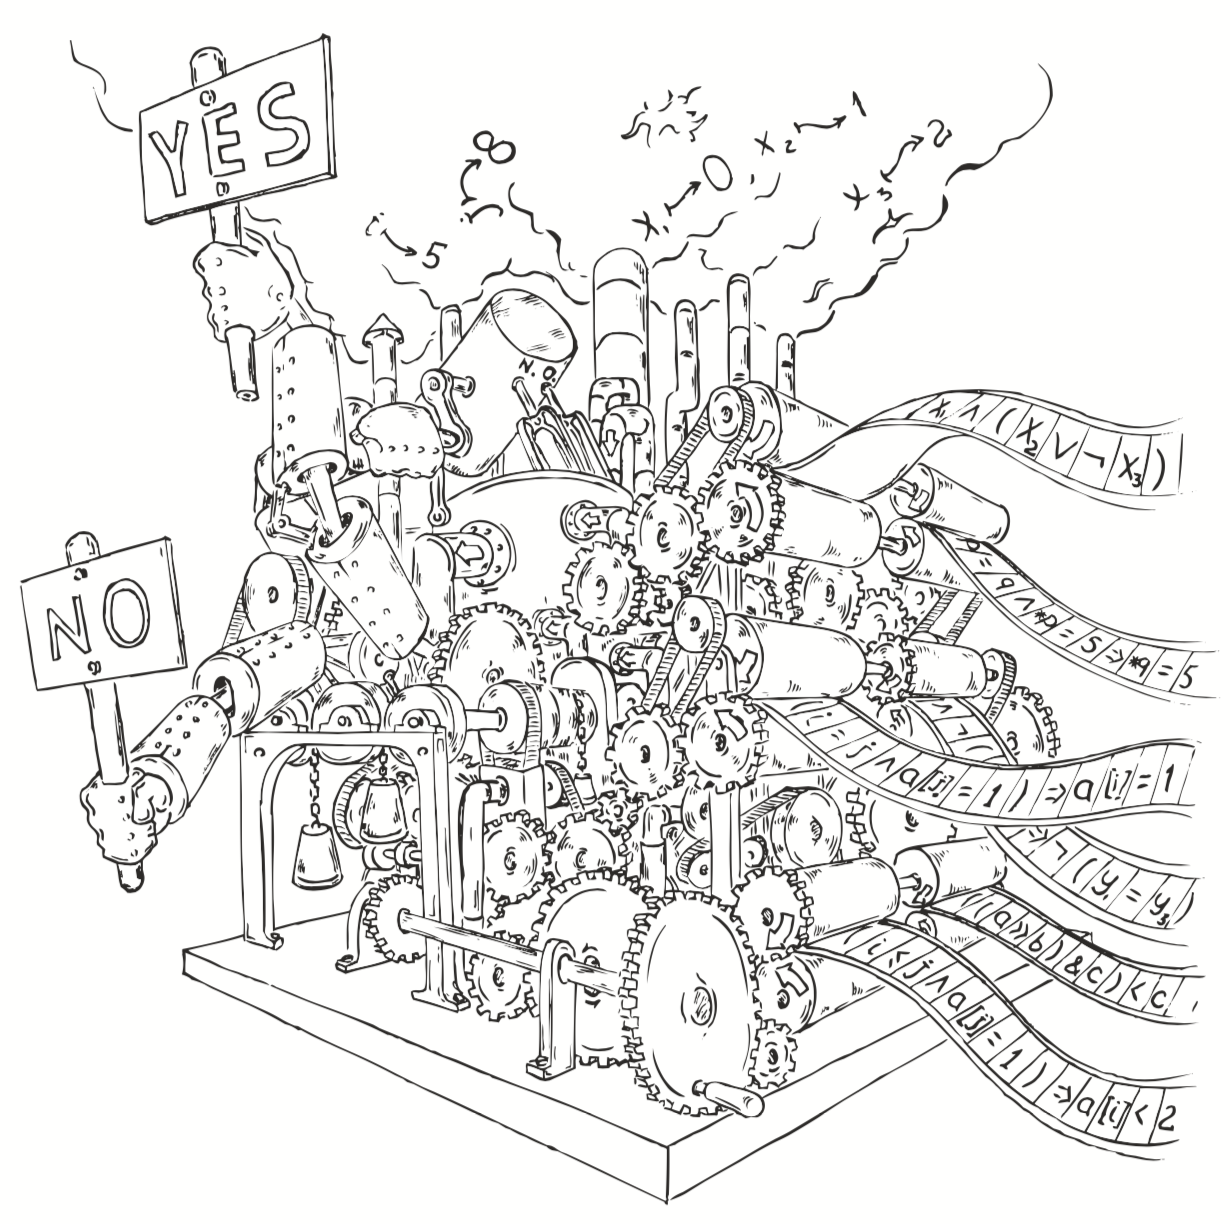
\includegraphics[scale=0.5]{../decision-procedure.png}
\end{frame}

\end{document}
